A/B testing can be applied in various ways to measure how effective improvements and updates are to a service. This essentially means utilizing 2 different groups of users to discover behavioural patterns and interpreting the result from the difference in performance. In GPP this might be used to improve the user interface by finding better color combinations and/or element positions. More importantly, tests could be run by teachers and researchers to determine which elements work and which don't.

One way of implementing this in GPP could be to divide a fraction of the user base into groups, expose them to changes and monitor its effects. For instance, testing the adventure map might show a significant increase in performance for group A whilst group B shows no change. Furthermore, change could possibly be seen in the second group---despite there being no change to the group itself---as the total amount of completed assignments increases in both groups.

Given that enough users participate in the A/B study, it can be shown with statistical significance that a gamification element is either beneficial or detrimental. In extension, this allows examiners to convince their faculties by showing them data proving its usefulness, allowing them to implement it into their courses.

The reason for this not yet being implemented is primarily that it requires the correct statistics to be available for extraction. Unfortunately, little work was devoted into statistics aggregation on the backend, meaning that until recently, implementing statistics-based features was very cumbersome. With a further developed statistics feature, implementing A/B testing should be feasible.

\subsubsection{A Twist}
\begin{wrapfigure}[14]{r}{6cm}
    \centering
    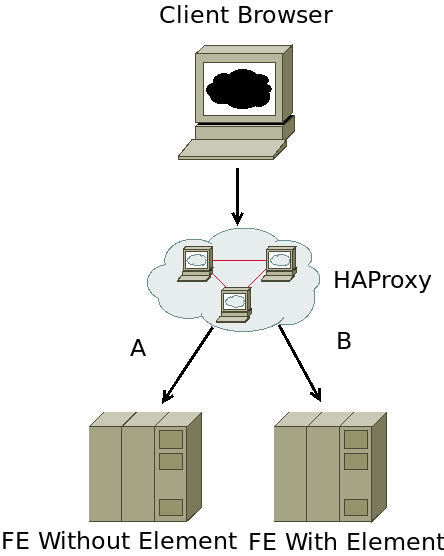
\includegraphics[width=.6\linewidth]{ab-loadbalanced.png}
    \caption{An alternative approach to A/B testing using the load-balancer.}
\end{wrapfigure}
Depending on what kind of statistics the A/B tests should determine, an alternative, more general approach could be taken. This works by implementing the testing \textit{on top of} the solution, instead of within, and may be easier to get started with. The drawback is that all tests would be done on a more coarse granularity.

Rudy Lee provides an example\cite{rudylee} for how this can be setup using the recommended HAProxy load-balancer. By first letting a balancing algorithm (round-robin, random or minimal-load) send users to a specific site and then setting a cookie to track and direct users on repeated visits, statistics like retention rate can be determined when doing site-wide changes. Unlike an A/B tester implemented inside the platform, this tool cannot capture changes done to single courses, only global ones, which limits the usefulness to educators.
